\section{Heuristische Evaluations-Funktion}
\label{sec:heuristic}
Dieser Abschnitt behandelt die heuristische Evaluations-Funktion, die zur Approximation des Nutzens eines Spielzustands
verwendet wird.

Optimalerweise würde die Evaluations-Funktion den tatsächlichen Nutzen einer Spielsituation bestimmen. Eine solche
Evaluations-Funktion ist zwar durch den Minimax Algorithmus gegeben, dieser kann jedoch aus offensichtlichen Gründen
nicht zum Einsatz kommen, da der Rechenaufwand hierbei identisch zu einer unbeschränkten Suche wäre.

Um den Nutzen verschiedener Spielzüge miteinander zu vergleichen, wird also eine weniger rechenaufwändige
Evaluations-Funktion benötigt, die diesen nur ausreichend gut annähert, statt den tatsächlichen Nutzen zu bestimmen.

\subsection{Anzahl der Steine}
\label{sec:disccount}
Ein primitiver Ansatz für eine Evaluations-Funktion bei dem Spiel Othello ist die Differenz der Anzahlen von eigenen
Steinen und gegnerischen Steinen auf dem Spielfeld, da diese am Ende über den Sieg entscheidet. Gegen Ende eines Spiels
könnte dieser Ansatz eine passende Bewertung liefern, allerdings kann es vor allem in der Anfangsphase sinnvoll sein,
weniger Steine zu haben. Viel wichtiger ist der Besitz von Ecken oder die Möglichkeit, neue Steine zu platzieren.
\cite[S.~7]{evaluationfunctions}

\subsection{Mobilität}
\label{sec:mobility}
Ziel der Mobilität ist es, dass der Spieler möglichst viele Steine platzieren kann. Dadurch kann dessen
Entscheidungsfreiheit maximiert, während die Freiheit des Gegners durch eine geringe Anzahl an Zügen eingeschränkt wird.
Es wird Unterschieden zwischen aktueller und potenzieller Mobilität, welche im Folgenden beschrieben werden.
\cite[S.~7f.]{evaluationfunctions}

\subsubsection{Aktuelle Mobilität}
\label{sec:theorycurrentmobility}
Die aktuelle Mobilität ist ein Maß dafür, wie viele mögliche Züge die Spieler gerade haben. Eine niedrige Anzahl an
möglichen Zügen ist häufig schlecht, da der Spieler gezwungen ist, einen weniger guten Zug zu machen. Als quantitatives
Merkmal kann zunächst die Differenz der möglichen Züge beider Spieler betrachtet werden. Allerdings ist eine Stellung
häufig besser, wenn man mehr mögliche Züge hat und der Gegner bei gleicher Differenz weniger mögliche Züge hat. Um diese
Tatsache zu berücksichtigen, kann eine nicht-lineare Funktion verwendet werden.
\cite[S.~7]{evaluationfunctions}

\subsubsection{Potenzielle Mobilität}
\label{sec:potmobility}
Neben der aktuellen Mobilität kann auch die potenzielle Mobilität betrachtet werden. Diese ist ein Indikator für die
mögliche Mobilität in folgenden Zügen. Michael Buro hat als aussagekräftigstes Merkmal die Summe aller Anzahlen freier
Felder um gegnerische Steine ausgemacht. Es wird also für jeden gegnerischen Stein überprüft, an wie viele freie Felder
dieser grenzt und die Summe darüber gebildet.
\cite[S.~8f.]{evaluationfunctions}

\subsection{Cowthello}
\label{sec:cowthello}
Die Ecken haben in Othello eine große Bedeutung, da sie nicht mehr durch den Gegner umgedreht werden können. Außerdem
ist es wahrscheinlich, dass der Spieler weitere angrenzende Felder erobern kann, die ebenfalls nicht mehr umgedreht
werden können. Die Cowthello-Heuristik ist aus dem gleichnamigen Online Othello Spiel Cowthello und gewichtet Felder
unterschiedlich.
\cite{cowthello}

Tabelle \ref{fig:cowthello} zeigt die Gewichtung der einzelnen Felder. Die Ecken sind am höchsten bewertet. Felder vor
den Ecken sind negativ bewertet, da durch diese der Gegner häufig die Ecke bekommt. Die Felder vor diesen sind wiederum
positiv bewertet, da sie Hilfsfelder sind, um später die Ecke zu bekommen. Außerdem sind Randfelder höher bewertet, da
diese nur durch ein weiteres Randfeld erobert werden können.

\begin{figure}[H]
    \centering
    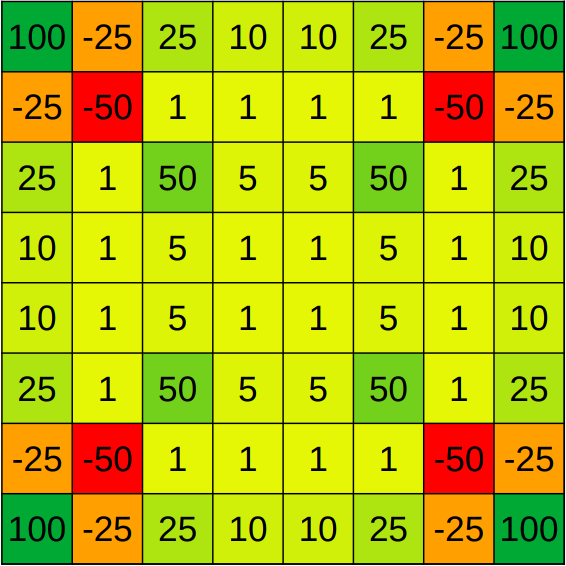
\includegraphics[width=\textwidth / 2]{cowthello}
    \caption{Gewichtung der Felder durch die Cowthello-Heuristik}
    \label{fig:cowthello}
\end{figure}

\subsubsection{Dynamische Gewichtung}
In Cowthello wird die Heuristik verändert, wenn Ecken belegt werden.
\cite{cowthello}

Das ist sinnvoll, da die an eine Ecke angrenzenden Felder negativ bewertet werden, weil der Gegner dadurch häufig die
Ecke bekommt. Wenn die Ecke bereits besetzt ist, spielt das keine Rolle mehr. Eine Möglichkeit, die Heuristik anzupassen, besteht darin, die Felder vor einer Ecke mit dem Absolutwert zu gewichten, sobald die Ecke besetzt ist.
